\documentclass{article}

% if you need to pass options to natbib, use, e.g.:
% \PassOptionsToPackage{numbers, compress}{natbib}
% before loading nips_2016
%
% to avoid loading the natbib package, add option nonatbib:
% \usepackage[nonatbib]{nips_2016}

% \usepackage{nips_2016}

% to compile a camera-ready version, add the [final] option, e.g.:
\usepackage[final]{nips_2016}

\usepackage[utf8]{inputenc} % allow utf-8 input
\usepackage[T1]{fontenc}    % use 8-bit T1 fonts
\usepackage{hyperref}       % hyperlinks
\usepackage{url}            % simple URL typesetting
\usepackage{booktabs}       % professional-quality tables
\usepackage{amsfonts}       % blackboard math symbols
\usepackage{nicefrac}       % compact symbols for 1/2, etc.
\usepackage{microtype}      % microtypography
\usepackage{graphicx}
\graphicspath{ {images/} }
\usepackage{floatrow}
\usepackage{float}

\title{Predicting IMDB Scores}

% The \author macro works with any number of authors. There are two
% commands used to separate the names and addresses of multiple
% authors: \And and \AND.
%
% Using \And between authors leaves it to LaTeX to determine where to
% break the lines. Using \AND forces a line break at that point. So,
% if LaTeX puts 3 of 4 authors names on the first line, and the last
% on the second line, try using \AND instead of \And before the third
% author name.

\author{
  M. Ugur~Gudelek\\
  Department of Computer Science\\
  TOBB University of Economics and Technology\\
  43 Sogutozu Avenue, Sogutozu, Ankara, 06560 Turkey \\
  \texttt{mgudelek@etu.edu.tr} \\
  %% examples of more authors
  %% \And
  %% Coauthor \\
  %% Affiliation \\
  %% Address \\
  %% \texttt{email} \\
  %% \AND
  %% Coauthor \\
  %% Affiliation \\
  %% Address \\
  %% \texttt{email} \\
  %% \And
  %% Coauthor \\
  %% Affiliation \\
  %% Address \\
  %% \texttt{email} \\
  %% \And
  %% Coauthor \\
  %% Affiliation \\
  %% Address \\
  %% \texttt{email} \\
}

\begin{document}
% \nipsfinalcopy is no longer used

\maketitle

\begin{abstract}
  Value of time is increasing for people day by day. Watching movies is a big stress-drop tool for these kind of people. Websites like IMDB or Rotten Tomatoes provides director or viewer rated movies. People sort that movies and watch one of them according to their choices. Prediction of score can be seen as machine learning problem.Therefore, in this project, we try to predict score of IMDB movies based on their properties.
\end{abstract}

\section{Introduction}

Providers like IMDB, Rotten Tomatoes, Metacritic allow viewers or users rate movies. Among these services, IMDB is the oldest and most popular one. They keep attributes of movies like gross, budget, where the movie made in, director review, etc. These information can be used to predict IMDB score which is a value between 0 to 10. In addition, Chuan Sun provides a dataset on Kaggle which is popular machine learning platform. We used this publicly provided dataset. Instead of using this dataset directly, we manipulate and fix some of the features to obtain better results. Several machine learning models are implemented and analyzed.

\section{Methods}
\subsection{Dataset}
The dataset consist of 5043 samples and 28 columns which consist of color, name of directors, actors, number of critic for reviews, duration, Facebook likes of director \& actors \& cast \& movie, gross, genres, movie title, number of votes by users, face number in poster, keywords of plot, IMDB link, number of user for reviews, language, country, content rating, budget, year, IMDB score, aspect ratio. Genres, country, language, keywords of plot, color are categorical values, others are continuous values.

\subsection{Feature preprocessing}
\subsubsection{Budget fixing}
In the budget column we have numerical values. However these numerical values need to be fixed before using because currency and inflation ratios were not handled properly.  We created a method which gets country and budget values then find currency code, exchange ratio with respect to currency code from the web to calculate new budget. We have fixed currency problem however we still have inflation problem. Therefore, we changed budget value using its year attribute to value on 1 January 2017. For instance, budget on 1920 is mapped to budget on 2017.

\subsubsection{One-hot encoding}
Categorical values should be replaced with their binary representation. This process is named as one-hot encoding. For instance, column with categories a,b,c needs to be 001,010,100. Performing one-hot encoding guaranties 2 euclidean distance between categories. Same distance means same importance between categories. Genres, country, language, keywords of plot and color features are replaced by new presentation.
\subsubsection{Names to average score mapping}
Names of directors and actors have 2500 and 6000 different values respectively. Using names as it is cannot give good result on evaluation. Therefore, we transform names with mean of previous movie.
\begin{equation}
	u_j=\frac {(\sum\limits_{i=1}^{N} v_i) - v_j}{N-1}
\end{equation}

in this equation u\textsubscript{j} represents the average IMDB score of director "u" without its j\textsuperscript{th} film. Moreover, each 'v' represents the each film of the director "u". In this equation 'N' denotes the number of films directed by the director "u". We subtract current IMDB score because scores need to be predicted not hard coded.

\subsubsection{Handling Nan}
Dataset has many Nan values because of problems in data retrieving and feature preprocessing. However, we don’t want to drop all samples which has Nan values. Nan values can be seen as classification problem. We create a K-Neighbor classifier and regressor for categorical and continuous values respectively. These estimators take all dataset as input. We select one feature and label it as target and other part of the dataset labeled as features. Features will be used to predict Nan valued targets. Estimators are trained with samples which has target values already. Although we fill bunch of Nan values with ease of KNN estimator, several values did not fixed and have Nan values still. However, clarifying these need to be done to run estimators smooth. Simply, dropping Nan values is done here. If we did not perform this operation we lost 2105 sample in the first place. However, we saved 990 Nan sample.


\subsection{Feature selection}

	Not all features have equally same importance. Some of them especially are meaningless indeed. Therefore we choose to drop such features before going deeper. Movie title, plot keywords and aspect ratio are dropped. 
	Curse of dimensionality affects estimations significantly. Therefore, we create a method to choose k-best feature from dataset. ExtraTree regressor is used for elimination of unimportant features. Importances of features are shown in ~\ref{importances_figure}. After first 10-12 features, importance significantly drops therefore we select first 11 feature as inputs of estimators.
\begin{figure}[H]
    \caption{Feature importances shows which features are important than others.}
    \centering
     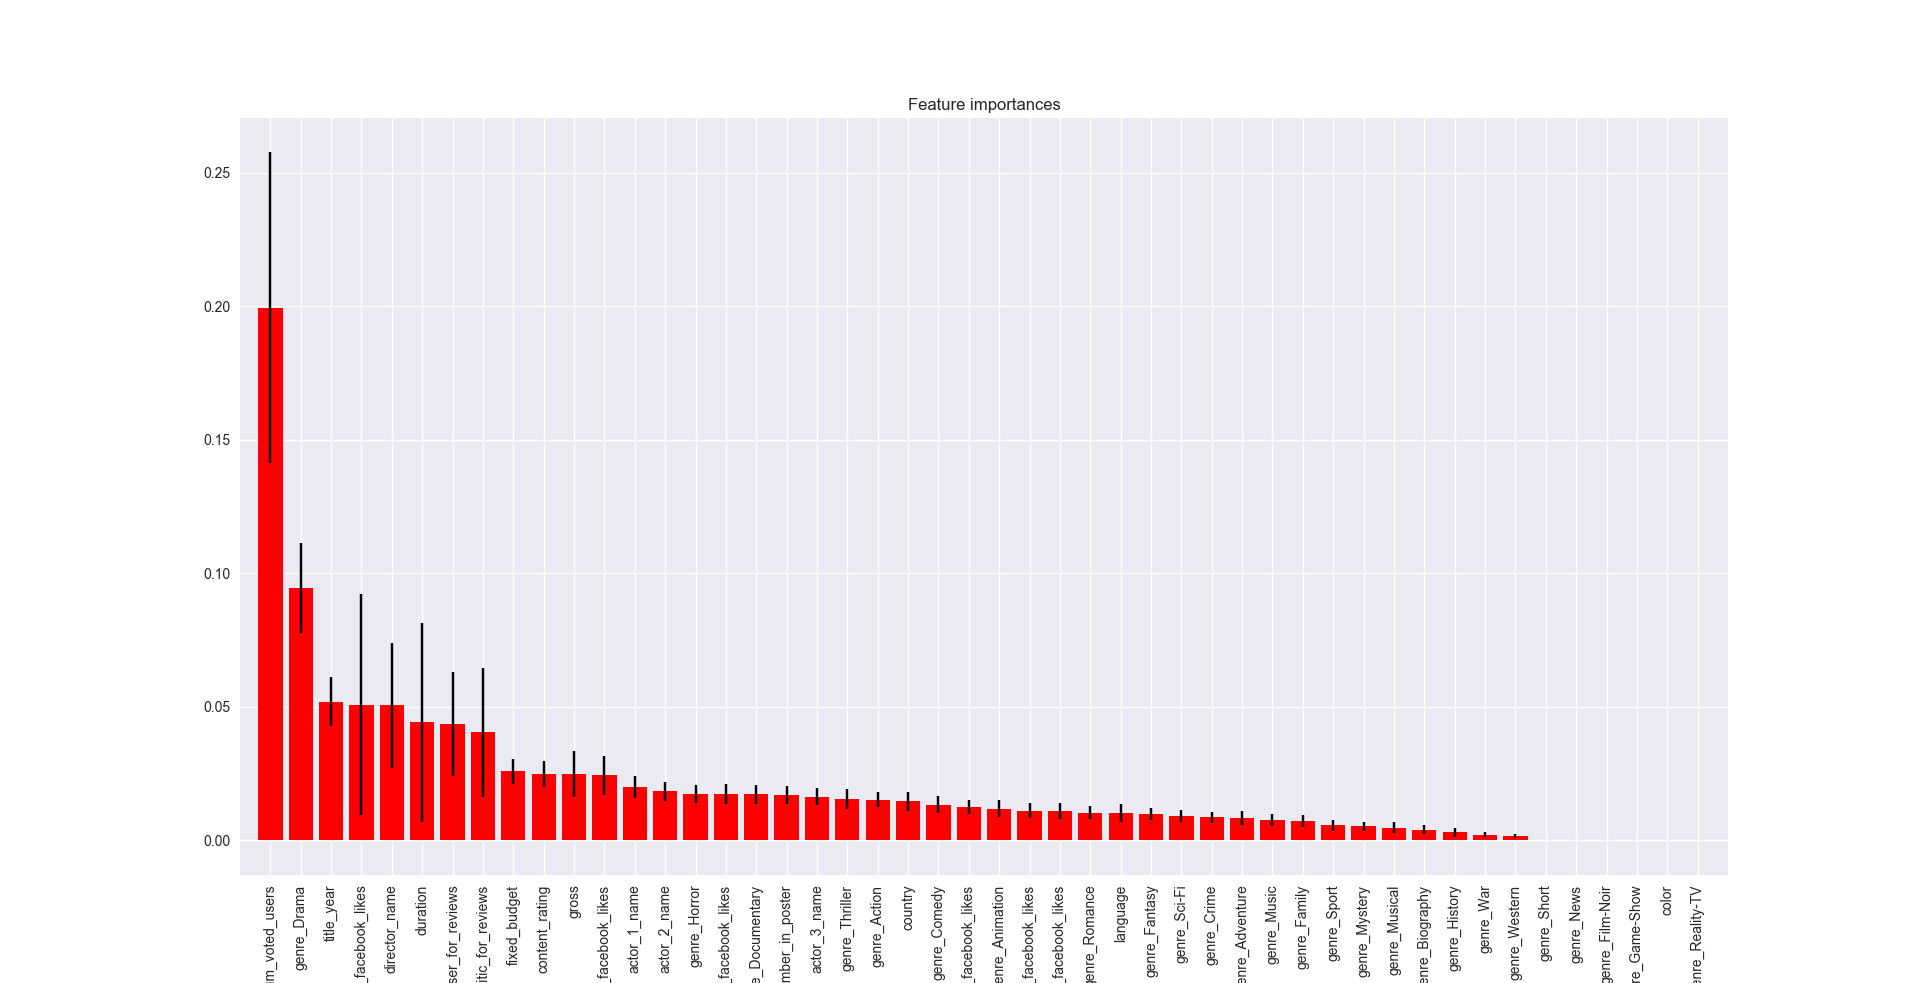
\includegraphics[width=10cm, height=5cm]{importances}
     \label{importances_figure}
\end{figure}
We try to visualize distribution of selected features over the IMDB score. Figure ~\ref{hexbin_figures} shows several samples from histogram of selected features. To be able to project 3D figure to 2D, we use hexbin method. Hexbin is a visualization process which gives deductible figure. The more bright hexagon the higher occurence they have. ~\ref{hexbin_figures}-c is the ground truth figure which is IMDB score vs IMDB score. As seen in ~\ref{hexbin_figures}-c, diagonal value from left bottom to right top shows high correlation as expected. ~\ref{hexbin_figures}-a is most important feature we have. It is the closest approximation of ~\ref{hexbin_figures}-c figure. Middle figure on the other hand has average importance and has circle-like shape. Distribution of brightness is correlated with precision accuracy.
\begin{figure}[H]
  \centering
  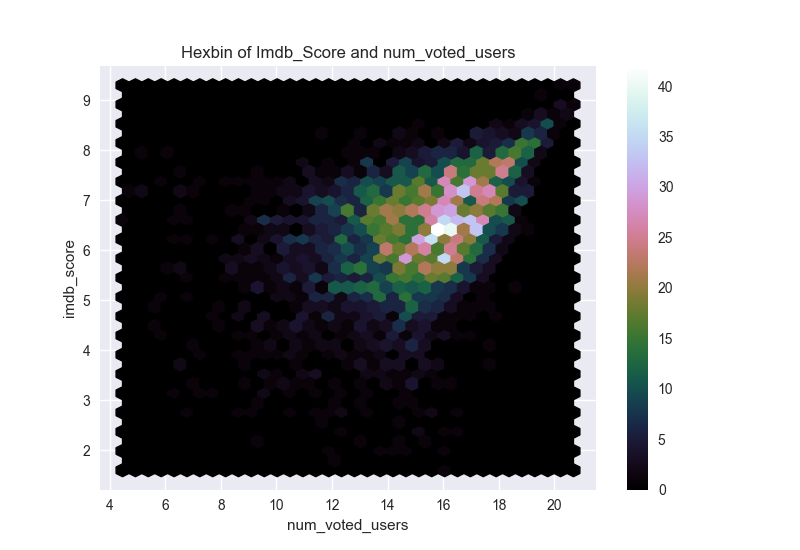
\includegraphics[width=4.5cm, height=4cm]{num_voted_users}
  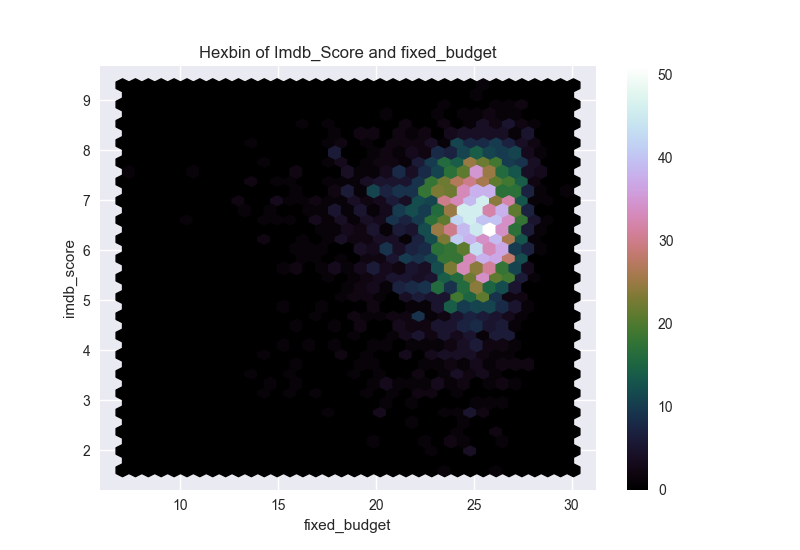
\includegraphics[width=4.5cm, height=4cm]{budget}
  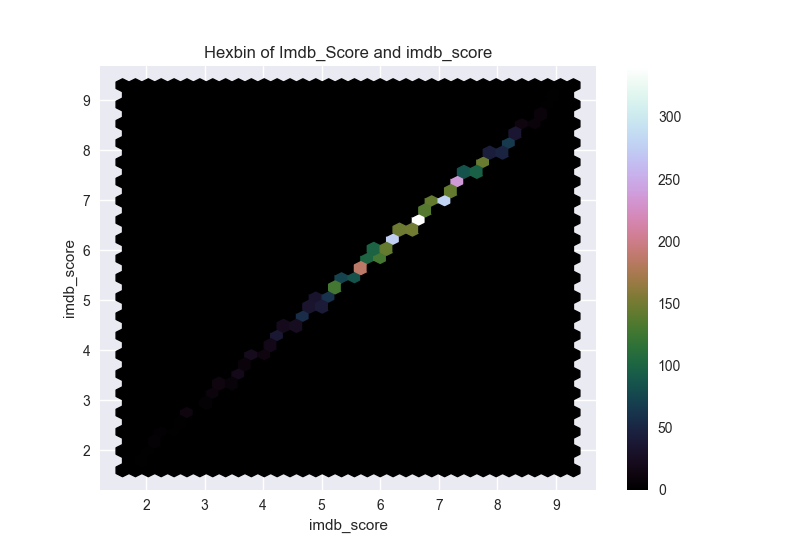
\includegraphics[width=4.5cm, height=4cm]{imdb_score}
  \caption{Histogram representation of several features vs IMDB score.}
  \label{hexbin_figures}
\end{figure}

Pearson correlation states that correlation between two variable is proportional to their pearson correlation coefficient. Equation ~\ref{eqn:pearson} shows true formula. We calculate all combinations among important features. Dark blue areas indicate higher correlation in figure ~\ref{fig:pearson}. Dropping highly correlated features is useful with respect to curse of dimensionality.
\begin{equation}
	\rho_{X,Y} = \frac{cov(X,Y)}{\sigma_X\sigma_Y}
    \label{eqn:pearson}
\end{equation}

\begin{figure}[H]
	\centering
    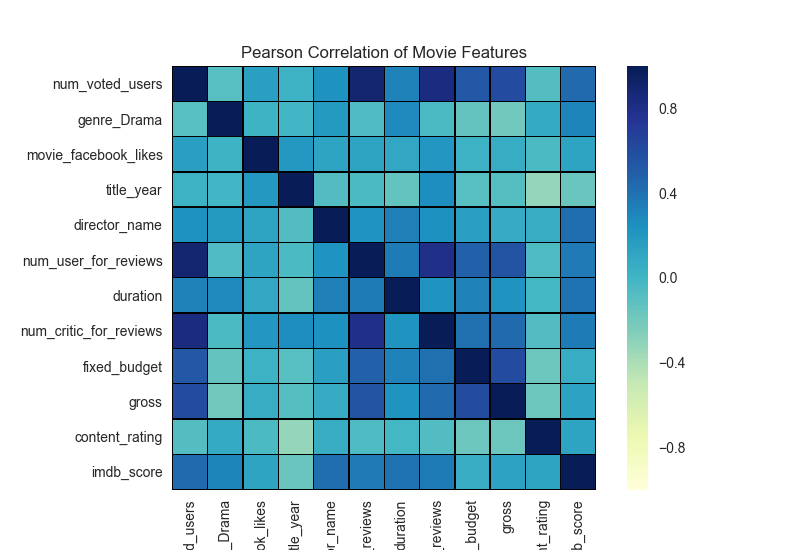
\includegraphics[width=10cm, height=6cm]{pearson}
    \caption{Pearson correlation coefficient visualization.}
    \label{fig:pearson}
\end{figure}

\subsection{Regression models}
We compare 5 different regression model which are support vector machines regressor, extra tree regressor, random forest regressor, linear regression, boosting regressor. To obtain better result we try to use ensemble models.
Number of estimators in forest models is 250. Taking opinion of 250 tree greatly reduce our variance and give better results. 
In SVR, 'rbf' kernel, 0.1 epsilon and 1.0 penalty factor is used. 

\section{Experimental Results}
MSE, MAE, custom designed score which return true when hit $\pm$1 of ground truth and R\textsuperscript{2} metrics used as score metrics. R\textsuperscript{2} shows performance of model. For the evaluation 5-fold cross validation approach is implemented. Cross validation is necessary because results can be luckily high or low because of choosing subsample of data. Cross validation corrects this phenomena. As expected most efficient estimators are ensemble methods because these methods decrease the variance by listening all individual tree inside them. Combining several methods to decrease volatility is the key in this concept.
Unoptimized SVR lacks of power of support vector machines. Therefore, in some cases linear regression model gives better results than SVR. 

Results can be seen ~\ref{result-table}

\begin{table}[H]
  
  \centering
\ttabbox{
  \caption{Comparison between estimators score\textsubscript{total} $\pm$1 denotes score within $\pm$1   range of true value, MSE denotes mean squared error, MAE denotes mean absolute error, R\textsuperscript{2} denotes	 coefficient of determination}
  \label{result-table}
}
{%
  \begin{tabular}{lcccc}
    \toprule
    \multicolumn{5}{c}{Estimator Comparison}                   \\
    \cmidrule{1-5}
    Name     & score\textsubscript{total} $\pm$1     & MSE 	& MAE	&R\textsuperscript{2}\\
    \midrule
    SVR					& 0.87  & 0.65	& 0.58	&0.43 \\
    Linear Regression   & 0.87 	& 0.61 	& 0.58	&0.47 \\
    Random Forest		& 0.92  & 0.58 	& 0.55 	&0.49 \\
    Extra Forest		& 0.92  & 0.54 	& 0.54 	&0.52 \\
    Boosting			& 0.92  & 0.53	& 0.53 	&0.53 \\

    \bottomrule
  \end{tabular}
  }%
  
\end{table}

\section{Conclusion}
\label{conclusion-section}
The problem of movie rating prediction is considered as machine learning
problem in this project. We have used public IMDB database and public exchange ratios to solve this problem. We run simple and complex regression algorithms which work within different domains. What we need is more samples from IMDB database to create more accurate estimators. This will highly improve our results. As a future work, we will collect more data on the web and optimize several estimators we have used. 

\section*{References}

\small

[1] Movies, TV and Celebrities. (n.d.). Retrieved April 03, 2017, from http://www.imdb.com/

[2] Your Home for Data Science. (n.d.). Retrieved April 03, 2017, from http://www.kaggle.com/


\end{document}


